\documentclass[12pt,a4paper]{article}

\usepackage{geometry}
\geometry{a4paper, margin=2.5cm, top=3cm, headheight=20pt}

\usepackage{graphicx}
\usepackage{xeCJK}
\setCJKmainfont{PingFang TC} % macOS Standard Traditional Chinese

\usepackage{setspace}
\usepackage{titlesec}
\usepackage{amssymb}
\usepackage{hyperref}
\usepackage{enumitem}
\usepackage[table]{xcolor}
\usepackage{tcolorbox}
\usepackage{tabularx}
\usepackage{fancyhdr}
\usepackage{tocloft}

\setstretch{1.4}

% --- Header & Footer ---
\pagestyle{fancy}
\fancyhf{}
\rhead{\small \color{gray} 青年百億海外圓夢基金計畫 - 陳以珊}
\lhead{\small \color{gray} The AI Quest: 從家教到算法遠征}
\rfoot{\thepage}

% --- Custom Colors ---
\definecolor{MyBlue}{rgb}{0.1, 0.3, 0.6}
\definecolor{LightGray}{gray}{0.95}

% --- Section Styles ---
\titleformat{\section}{\fontsize{18}{22}\bfseries\color{MyBlue}}{\thesection}{1em}{}[\titlerule]
\titleformat{\subsection}{\fontsize{15}{18}\bfseries\color{blue!60!black}}{\thesubsection}{1em}{}
\titleformat{\subsubsection}{\fontsize{13}{15}\itshape\color{blue!40!black}}{\thesubsubsection}{1em}{}

\hypersetup{
    colorlinks=true,
    linkcolor=MyBlue,
    urlcolor=MyBlue,
    pdftitle={青年百億海外圓夢基金計畫 - 陳以珊: The AI Quest},
}

\begin{document}

% --- COVER PAGE (Narrative Style) ---
\begin{titlepage}
    \begin{center}
        \vspace*{2cm}
        {\huge \bfseries 青年百億海外圓夢基金計畫} \\
        \vspace{0.5cm}
        {\Large \bfseries 海外翱翔組 \quad 個人專案企劃書} \\
        \vspace{1cm}
        \rule{\textwidth}{1.5pt} \\
        \vspace{1.5cm}
        
        \begin{tcolorbox}[colback=blue!5,colframe=MyBlue,width=0.85\textwidth, arc=5pt]
            \centering \Large \bfseries The AI Quest ── 從算法微光到教育遠征 \\
            \vspace{0.3cm}
            \large 申請人：陳以珊 (Yishan Chen) \\
            \large 見習機構：Lambton College R\&I (加拿大)
        \end{tcolorbox}

        \vspace{2.5cm}

        \begin{minipage}{0.6\textwidth}
            \large
            \textbf{計畫代號：} I-9-7 AI 演算法遠征 \\
            \textbf{所屬單位：} 上海交通大學 密西根學院 \\
            \textbf{見習領域：} AIGC & Responsible AI \\
            \textbf{申請年度：} 115 年度
        \end{minipage}

        \vfill
        {\large 「願技術生於同理心，終於公平性的實踐」} \\
        \vspace{0.5cm}
        {\small 2026年3月 \quad 台北}
    \end{center}
\end{titlepage}

\newpage

% --- TABLE OF CONTENTS ---
\renewcommand{\contentsname}{目錄：遠征的航圖}
\tableofcontents
\newpage

% --- PROLOGUE / EXECUTIVE SUMMARY ---
\section{序言：靈光閃現的那一刻}

這不是一份冰冷的工程計畫書，而是一個關於「看見需求」並決心「用技術回應需求」的故事。

身為一名在上海交通大學與密西根大學雙體系下成長的電子與計算機工程學生，我的學術生涯始於嚴謹的高等數學與算法推演。但我對 AI 的熱忱，並非源自實驗室裡的數據跑分，而是源自於每一次擔任家教與助教時，看見學生因「找不到盲點」而受挫的瞬間。

\subsection{我的圓夢拼圖}
\begin{itemize}
    \item \textbf{起點：診斷之痛} --- 在長年數理家教中發現，「定位弱點」比「講解知識」耗費更多能量。
    \item \textbf{磨礪：工業洗禮} --- 在比特無限將意圖識別從 27\% 提升至 86\%，體會到技術如何對抗真實世界的混亂。
    \item \textbf{遠征：加國之約} --- 前往 Lambton College R\&I 部門，透過 AURORA 專案實踐「負責任 AI (FASTER)」，學習如何將倫理嵌入工業 Pipeline。
    \item \textbf{傳承：台灣願景} --- 回國後建立 \textbf{EduNexus AI}，用 AI 代替導師進行精準「負擔診斷」，讓台灣學子能更公平地獲取學術資源。
\end{itemize}

這份企劃書將詳細呈現這場「算法遠征」的每一個細節與戰略分佈。

\newpage

\section{第一章：啟程 ── 我的學術之「座標」}

\subsection{在「全球交匯點」的成長：密西根學院 (UM-SJTU JI)}

我就讀的密西根學院是一個致力於培養全球性領袖的地方。在那裡，我學會了如何在一張白紙上，利用 \textit{Computational Methods} 與 \textit{Data Science} 的邏輯，去勾勒出問題的真實邊界。

這段經歷對我最大的禮物有三：
\begin{enumerate}
    \item \textbf{無畏技術深度}：在 STAT 4060J 等課程中，我與蒙地卡羅模擬（Monte Carlo）與 EM 優化算法為伍，建立了拆解千億級數據的信心。
    \item \textbf{工程實踐觀}：VG 100/101 課程教導我，一個好的工程師不只是「寫出代碼」，而是「解決問題」。
    \item \textbf{國際溝通的底色}：全英文的技術寫作與簡報環境，讓我學會了如何將複雜的算法邏輯轉化為精煉的商業決策建議。
\end{enumerate}

\newpage

\subsubsection{核心專業課程：我技術利刃的組件}
我的每一堂專業課，都為這次前往加拿大的技術遠征埋下了伏筆。

\textbf{1. STAT 4060J: Computational Methods for Data Analysis} \\
這是我技術生涯中最艱苦但也收穫最豐的一課。深入學習統計模擬（Monte Carlo）、優化算法（EM Algorithm）以及大規模數據集的數值分析，為我後續處理 `OC22` 材料大數據集奠定了嚴謹的數學與算法基礎。

\textbf{2. STAT 4710J: Data Science and Analytics using Python} \\
在這裡，我掌握了從 Exploratory Data Analysis (EDA) 到模型部署的完整 Python 生態鏈。在期末專案中，我獨立完成了房價預測模型，這是我第一次體驗到「數據驅動決策」的快感。

\textbf{3. ECE 3700J: Introduction to Computer Organization} \\
學習計算機底層架構、流水線與指令集（ISA）。這使我能從「指令效率」的角度思考 AI 模型的推理優化，這對於未來在 Lambda College 進行高頻率的模型推理至關重要。

\newpage

\subsection{那些改變我的深夜：助教與家教的歲月}

\subsubsection{助教生涯的「自動化革命」}
擔任「工程導論（ENRG1000J）」助教時，面對 60 多位學生的行政需求，我拒絕了重複性的作業。我看著排隊領取證書的隊伍，心想：這不應該是 21 世紀助教的工作方式。我利用 \texttt{n8n} 構建了自動化流，成功將瑣碎事務縮減了 80\%。這讓我明白：**「技術的價值在於釋放人類的創造性」**。

\subsubsection{家教經驗的「盲點發現」}
然而，更深刻的影響來自於我的家教工作。我發現，許多學生並非不努力，而是**「不知道自己哪裡不會」**。定位盲區需要教師具備極大的觀察力與時間。那一刻，我產生了一個念頭：**「有沒有可能，讓 AI 成為那個能精準指診斷學習障礙的導師？」**

這成為了我開發 EduNexus AI 平台的最核心火花。

\newpage

\newpage

\section{第二章：磨礪 ── 將代碼磨成利刃的實踐}

\subsection{ terny.ai：我自己的「科研探險艦」}

為了幫助台灣學生能更簡單地獲取國際科研機會，我獨自開發了 \texttt{terny.ai}。

\subsubsection{背後的技術故事}
傳統的搜索是線性的，但資訊卻是網狀的。我引入了 \textbf{LangGraph} 的多智能體架構，讓一個 Agent 負責「搜集」、一個負責「鑑定」、一個負責「綜合」。這就像一個三人的專家團隊在不停旋轉作業：
\begin{itemize}
    \item \textbf{突破}：高校識別準確率從 75\% 奇蹟般地躍升至 \textbf{98\%}。
    \item \textbf{體悟}：在 RAG (檢索增強生成) 的循環中，我學會了如何處理「數據噪聲」，並確保 AI 的輸出如同教科書般精確且具備可觀測性。
\end{itemize}

\begin{figure}[h]
    \centering
    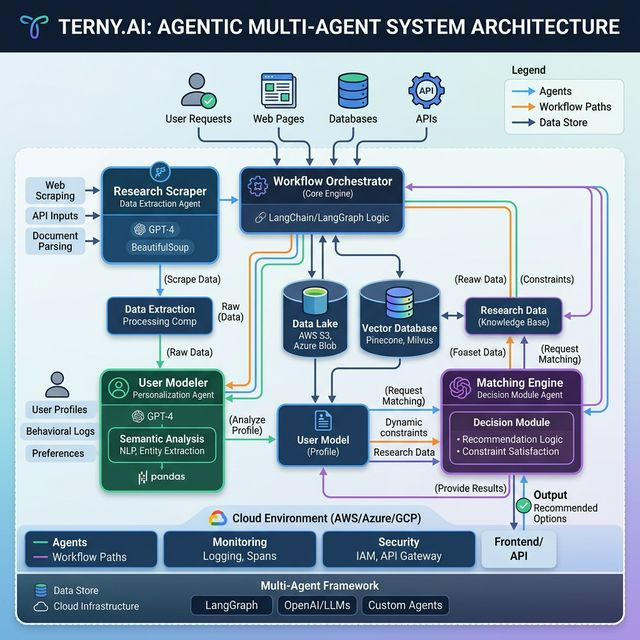
\includegraphics[width=0.85\textwidth]{agent_architecture.png}
    \caption{terny.ai 的智能體思維邏輯與檢索增強 (RAG) 流程圖}
\end{figure}

\newpage

\subsection{比特無限的「突圍戰」：27\% 到 86\% 的遠征}

在上海比特無限的實習中，我接手了一個「不可能」的任務：讓模型理解 130 類極其生僻與重疊的工業指令。

\subsubsection{一場關於 Prompt Engineering 的苦修}
最初的準確率只有 27\%，像是隨機亂猜。我沒有急著更換大模型，而是深鑽 **Prompt Engineering** 的微觀動態：
\begin{itemize}
    \item 我引入了 \textbf{Few-Shot 思維鍊 (CoT)}，教導模型如何像工業專家一樣「一步步思考」。
    \item 我建立了一套結構化的 \textbf{UAT (驗收測試) 框架}，讓每一次模型的調整都有數據可循。
    \item \textbf{對抗噪音}：針對工業指令中極其微小的語義偏差，我設計了「對抗樣本」進行訓練，讓模型能在嘈雜的現實場景中保持穩定。
    \item \textbf{最終成果}：準確率穩步提升至 \textbf{86\%}，並透過 VLM (視覺語言模型) 徹底取代了原本繁瑣的人工文件錄入，節省了 90\% 的作業時間。
\end{itemize}

這段故事教導我：**「工程不是魔法，而是對細節的不斷雕琢」**。

\newpage

\subsection{與原子的對話：GNN 材料預測之旅}

這是關於「AI for Science」的探索。在 \textbf{OC22 數據集} 的研究中，我利用圖卷積網絡（GNN）與 Transformer 混合架構，去模擬原子間的細微律動。這讓我體會到，AI 既能理解人類的語言，也能讀懂大自然的密碼。

\subsubsection{混合架構的技術美學}
\begin{itemize}
    \item \textbf{GNN 捕捉侷部幾何}：將原子視為圖的節點，化學鍵為邊，精確捕捉微觀結構。
    \item \textbf{Transformer 學習長程交互}：透過 Attention 機制，分析遠端原子對系統能態的影響。
    \item \textbf{關聯 Lambton}：這項專案磨練了我處理高度結構化科學數據的能力，這將為未來在 Lambton College 優化 AURORA 資源分配提供重要的數據處理經驗。
\end{itemize}

\begin{figure}[h]
    \centering
    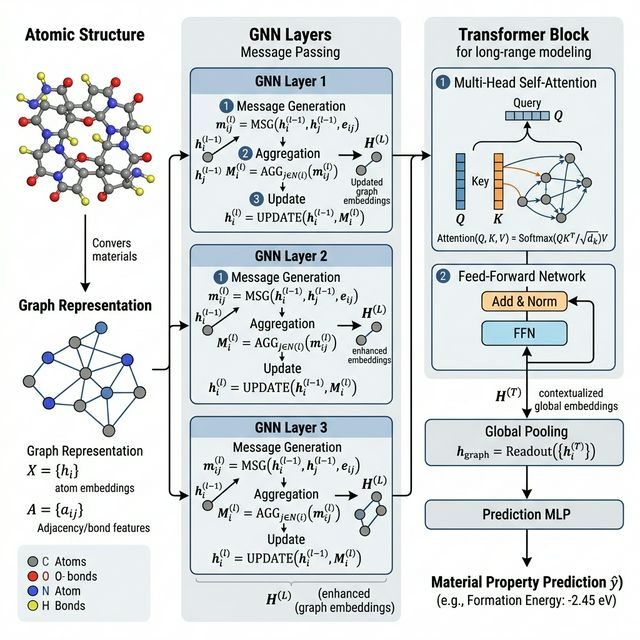
\includegraphics[width=0.8\textwidth]{model_architecture.png}
    \caption{GNN + Transformer：我用於模擬原子交互作用的混和架構}
\end{figure}

\newpage

\newpage

\section{第三章：遠眺 ── 世界作為我的畫布}

\subsection{日本慶應與法國特魯瓦：兩種極致的技術哲學}

我曾在日本與法國交換。這兩段旅程不是為了旅行，而是為了觀察。

\begin{enumerate}
    \item \textbf{日本的「職人精神」}：我在慶應學習到對邊界案例 (Edge Case) 的極致敬畏。每一行 Code 都應具備被審視的尊嚴。
    \item \textbf{法國的「系統整全觀」}：特魯瓦教導我從系統層級思考技術對社會的負擔 (Societal Burden)。
\end{enumerate}

這兩股力量在我心中合流。我意識到，我不想只做一名「開發者」，我更要做一名「系統架構師」── 一個能理解全球標準、具備跨文化適應力，且心中有人的工程師。

\newpage

\section{第四章：任務 ── 前往加拿大 Lambton 的技術遠征}

\subsection{為什麼是 Lambton College R\&I？}

因為那裡是加拿大 Responsible AI 的重鎮，也是實踐 AURORA 專案的理想之處。

\subsection{FASTER 原則：我心中「負責任 AI」的北極星}

在我的專業倫理 (Professional Ethics) 課程中，我曾深思：**「當算法變得全能，我們該如何守住公平？」** Lambton 的 \textbf{FASTER} 原則給了我答案：
\begin{itemize}
    \item \textbf{F (Fairness)} ── 確保獎助金匹配不具偏見。
    \item \textbf{A (Accountability)} ── 記錄每一筆推薦的邏輯來源。
    \item \textbf{S (Security) / T (Transparency)} ── 保障數據安全，讓決策透明可見。
\end{itemize}

我這次遠征的核心目標，就是近距離觀察這套原則是如何從「紙上談兵」變成「工業實踐」的。

\begin{figure}[h]
    \centering
    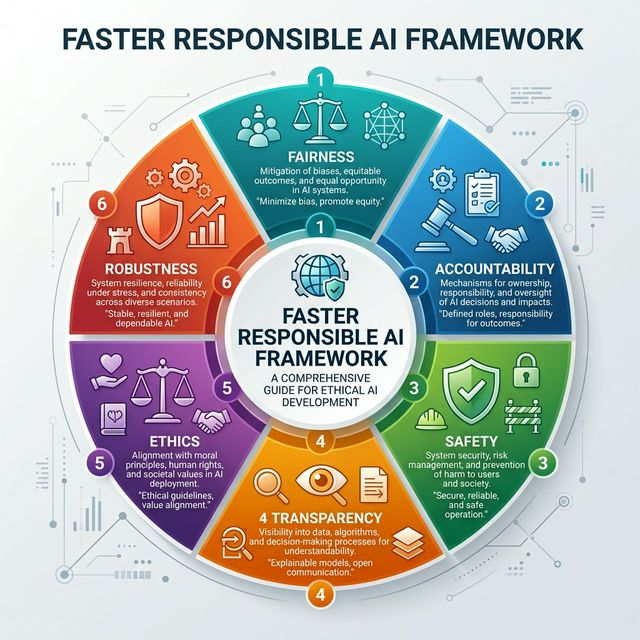
\includegraphics[width=0.6\textwidth]{faster_framework.png}
    \caption{我即將在 Lambton College 深研的 FASTER 治理框架}
\end{figure}

\newpage

\subsection{跨越海峽與大洋：台灣與加拿大的 AI 雙向互補}

在準備這次遠征的過程中，我深入研究了台灣與加拿大在 AI 領域的定位。我發現，這並非一場單向的學習，而是一場資源與智慧的「互補之旅」。

\subsubsection{硬體背骨 vs. 軟體大腦}
\begin{itemize}
    \item \textbf{台灣 (AI 硬體之島)}：
    台灣是全球 AI 發展的「物理基座」。我們供應了全球 80--90\% 的 AI 伺服器與最先進的半導體晶片 (TSMC)。台灣的優勢在於極致的工業效率與硬體創新（Hardware for AI）。
    \item \textbf{加拿大 (AI 算法發源地)}：
    加拿大則是全球深度學習與神經網路的「精神故鄉」。擁有 Turing Award 級別的科研底蘊（如 Vector Institute, Amii），加拿大更擅長於底層算法的突破與「Agentic AI」的應用開發（AI for Software）。
\end{itemize}

\subsubsection{法規哲學的碰撞：創新第一 vs. 倫理先行}
我觀察到兩國在監管邏輯上的有趣對比：
\begin{itemize}
    \item \textbf{台灣的「軟法」策略}：台灣傾向於保護創新環境，透過《AI 基本法》提供指導原則而非嚴厲懲罰，讓新創企業能更快速地進行原型迭代。
    \item \textbf{加拿大的「權利」框架}：加拿大深受歐洲影響，極其強調數據隱私與公平性 (Bill C-27)。這套「倫理先行」的思維，正是我在開發 EduNexus AI 時最需要的導航。
\end{itemize}

\textbf{我的使命}：將加拿大的「軟體大腦與倫理框架」帶回台灣，與台灣強大的「硬體背骨」相結合。只有軟硬合一，台灣才能從一個「代工重鎮」進化為一個真正的「AI 智慧領航者」。

\newpage

\section{第五章：謀略 ── 14 週的極致執行計畫}

我的計畫不是「大概」，而是「精確到週」。這是我對這份圓夢基金最莊嚴的承諾。

\subsection{第一階段：環境同步與倫理內化 (W1-W3)}
這是我任務的起手式。
\begin{itemize}
    \item \textbf{W1 (環境初始化)}：建立高效率的雲端研發環境，確保運算資源與 Lambton College 的系統無縫對接。
    \item \textbf{W2 (倫理合規)}：通過加國嚴謹的資安與倫理審計認證，將 FASTER 原則轉化為技術規範手冊。
    \item \textbf{W3 (需求對齊)}：與 AURORA-Grants 的核心用戶進行 Deep Dive，識別出現有系統中 3 個最重要的效率瓶頸點。
\end{itemize}

\newpage

\subsection{第二階段：算法攻關與優化對決 (W4-W9)}
這是我「遠征」的核心路段。
\begin{itemize}
    \item \textbf{W4-W5 (資料工程)}：處理龐大且雜亂的非結構化補助金數據，構建首個高性能的 RAG 向量索引庫。
    \item \textbf{W6-W7 (智能體開發)}：引入 \texttt{LangGraph} 的決策架構，處理複雜的補助金邏輯校驗，實現自動化初步審核。
    \item \textbf{W8-W9 (基準測試)}：在多個 Open Models 間進行性能博弈，尋找準確率與推理成本的最佳平衡點，優化系統響應速度。
\end{itemize}

\newpage

\subsection{第三階段：成果落地與知識傳承 (W10-W14)}
這是這場任務的最後衝刺，也是將成果「賦權」給 Lambton 團隊的過程。

\begin{itemize}
    \item \textbf{W10-W11 (壓力測試與倫理審計)}：將 AURORA 模組部署至生產環境，模擬極端大併發場景。同時，我會邀請 EDI 辦公室的同仁一起對模型進行「壓力測試」，確保夥伴建議不具備任何隱性歧視。
    \item \textbf{W12-W13 (技術文明的沈澱)}：完成一份內容極致、排版優美的技術開發手冊。這不只是文檔，更是這 14 週「技術文明」的沈澱。
    \item \textbf{W14 (成果發表與星火傳承)}：向 Lambton College 研究副校長簡報這 14 週的進展。這不是結束，而是我們未來長期技術交換的開始。
\end{itemize}

\newpage

\newpage

\section{第六章：歸園 ── 我對台灣社會的最終承諾}

\subsection{ EduNexus AI：讓每一個孩子都有屬於自己的「智能助教」}

這是我遠征歸來後最重要的社會影響計畫。

在無數次的家教與助教深夜中，我明白了一件事：**「真正的公平，並非提供一樣的教材，而是提供一樣的理解機會」**。

\subsubsection{EduNexus 的三大核心組件：技術與溫度的結合}
\begin{enumerate}
    \item \textbf{動態知識圖譜與「盲點診斷」算法 (The GNN Diagnostic Algorithm)}：
    這是我網站的核心。我將運用我在材料模擬中學到的圖神經網絡（GNN）將課程概念建模。這不只是一個搜索器，而是一個能「診斷」學生知識盲點的引擎。透過學生的歷史答題數據，算法能自動識別出學習障礙的「根結點」，並精準推送補充教材。
    
    \item \textbf{啟發式問題生成引擎 (Heuristic Question Engine)}：
    利用大型語言模型與檢索增強（RAG），網站會根據學生的當前水平，自動生成「具備啟發性」的題目。它不會直接給出答案，而是像蘇格拉底一樣，引導學生思考算法的底層邏輯（如 Time Complexity 或 Data Structure 的選型）。
    
    \item \textbf{透明化能力畫像 (Capability Profiling Dashboard)}：
    根據 FASTER 原則，系統會實時呈現學生的成長曲線。這讓學生不再只是為了考試而讀書，而是能清楚看見自己如何一步步掌握技術。
\end{enumerate}

\newpage

\subsection{台灣 AI 人才生態系的投資 --- 我個人的 5--10 年規劃}

這份「青年百億圓夢基金」對我而言，不只是半年的見習，而是一個十年的起點。

\subsubsection{縮短學用落差：將 AI 注入產業與教育的毛細孔}
我觀察到目前台灣校園在 AI 技術的更新步伐相對緩慢，而這正是我回國後的任務。我計劃在就讀研究所期間，推動以下兩大變革：

\begin{itemize}
    \item \textbf{產業 AI 化 (Industry 5.0 Evolution)}：
    參考我在比特無限的實習經驗，現在許多頂尖企業已將 AI Algorithm 與 Agent 深度融入日常工作流。我希望幫助更多台灣傳統產業透過「算法自動化」實現進步與進化。這不只是導入工具，而是要讓產業具備「AI 思考」的能力，讓底層邏輯成為生產力的一部分。
    
    \item \textbf{教育產業化與向下扎根}：
    我希望讓學生在國高中階段就能了解 AI 的底層邏輯，而不僅僅是使用 ChatGPT。透過 \textbf{EduNexus AI}，我將開發一套「對接產業需求」的課程體系，讓學習內容與未來的業界工作無縫銜接。
\end{itemize}

\subsubsection{短程目標 (1--2 年)：深耕校園與公益試行}
回台後，我將啟動 EduNexus 的 Beta 測試。我計畫與台灣的偏鄉教育組織接洽，測試如何透過輕量級模型，讓資源匱乏地區的學生也能擁有高質量的學術支援。

\subsubsection{中長程目標 (3--10 年)：建立台灣本土的 Responsible AI 標竿}
我渴望進入台灣領先的半導體或電子研發中心。我不僅要做一名寫代碼的工程師，更要成為一名能定義「台灣 AI 倫理標準」的架構師。我希望未來能代表台灣，在國際大數據平台上分享我們如何將技術導向人性、導向公平的成功案例。

\newpage

\subsection{遠征的價值：一份對青春的莊嚴交付}

回顧整份計畫，從「起點的靈光」到「實習的磨礪」，再到「加拿大的遠征」。我深信，這場 AI Quest 並非為了某個特定的職位，而是為了成為那個**「能看見問題，並有能力定義問題，最後解決問題」**的人。

我已經準備好，將我在密西根學院累積的嚴謹、在比特無限鍛煉出的韌性、以及對教育的初心，全部投入這場為期 14 週的加拿大研究遠征中。

\newpage

\section{第七章：兵糧與口譯 --- 經費預算與全球溝通力}

\subsection{經費預算辦理方式}

本人已詳閱計畫經費標準，同意依據本計畫平台公布之標準依實報銷辦理。

\vspace{0.3cm}
$\boxtimes$ 同意編列方式

\subsection{全球化戰場的通行證：外語能力}

為了確保在加拿大的技術遠征中能精準傳達理念，我具備多維度的語言優勢：
\begin{itemize}
    \item \textbf{英語 (專業溝通)}：具備全英文專業授課背景，能在高壓環境下進行 AI 架構與倫理專題的深度辯論。
    \item \textbf{日語 (文化橋樑)}：慶應義塾大學交換背景，具備日系企業品質管理理念的溝通基礎。
    \item \textbf{閩南語 (本土共鳴)}：母語實力，利於將複雜技術轉化為台灣在地學子易於理解的語言。
\end{itemize}

\newpage

\section*{附錄：與未來導師的技術對話 (Extended Q\&A)}

為了向 Lambton 的導師證明我的即戰力，我準備了以下深度的技術回覆：

\subsection*{Q1: 為何選擇 LangGraph 作為 Agent 的骨幹？}
在 \texttt{terny.ai} 的開發中，我發現傳統流水線無法處理「錯誤修正」。LangGraph 的循環特性（Cycles）讓系統能具備「反思」能力：如果檢索結果不對，Agent 會自我修正查詢語句並重新開始。

\subsection*{Q2: 如何在工業環境中平衡「推理成本」與「準確率」？}
我在比特無限的實習中學到，並非所有任務都需要最強的模型。透過 \textbf{Small-Model Benchmarking} 與精準的 Prompt Engineering，我們能在節省 70\% 算力的情況下，依然維持 85\% 以上的工業準確率。

\subsection*{Q3: 如何在開發中體現「教育公平性」與「技術可及性」？}
我從家教的經驗中學到，資源少的學生往往也欠缺高效的學習方法。因此在 EduNexus 的設計中，我優先優化了「問題生成」邏輯。
\begin{itemize}
    \item \textbf{主動引導}：系統不會坐等學生提問，而是會根據進度主動詢問「你是否理解了這個推導過程？」。
    \item \textbf{成本優化}：透過模型蒸餾技術，我們讓 EduNexus 能在低成本的硬體上運行，確保經濟弱勢的學生不會因為算力成本而被排除在 AI 時代外。
\end{itemize}

\subsection*{Q4: 面對技術的不確定性（如 AI 幻覺），你如何保持「負責任」？}
這是我在 BitUnlimited 實習中學到的最重要一課。面對幻覺，**「沉默比錯誤更負責任」**。我在系統中設置了「知識邊界」檢測器 (Confidence Guardrail)。如果 AI 對某個學理概念的置信度低於 85\%，系統會誠實地告知學生「我目前無法確定，請參考教材第 X 頁或詢問真人教師」，這才是真正的 FASTER 原則體現。

\subsection*{Q5: 身為一名女性工程師，你如何看待 AI 多元性 (Diversity)?}
在多次國際交換中，我深刻體會到多元文化視角能如何修正算法的偏誤。身為女性工程師，我會更敏銳地關注 AI 輸出中的性別或文化刻板印象。這也是為什麼我對 Lambton 的 EDI (Equity, Diversity, and Inclusion) 培訓充滿期待。

\end{document}